\textbf{MTP:} Have small, lightweight models that predict multiple steps ahead
\begin{columns}[T]
\begin{column}{0.55\textwidth}
\centering
\includegraphics[page=46,trim=39 124 319 114,clip,width=\linewidth]{figure/cs336-l4.pdf}\\
{\scriptsize (But they only do MTP with one token ahead)\hfill [Deepseek v3]\par}
\end{column}
\begin{column}{0.43\textwidth}
\centering
\includegraphics[page=46,trim=413 106 35 97,clip,width=\linewidth,height=72pt,keepaspectratio]{figure/cs336-l4.pdf}\\
{\raggedleft\scriptsize [EAGLE]\par}
\end{column}
\end{columns}
\begin{center}
\includegraphics[page=46,trim=224 4 213 323,clip,width=\linewidth,height=32pt,keepaspectratio]{figure/cs336-l4.pdf}
\end{center}
\vspace{-6pt}
{\raggedleft\footnotesize (See paper for ablations)\par}
